\documentclass[t]{beamer}
\usepackage{mathtools}
\usepackage{tikz}
\usepackage{pgfplots}
\usepackage{ifthen}
\usepackage{calc}
\usepackage{datatool}
\usepackage{datapie}
\usetikzlibrary{arrows,backgrounds,shapes,matrix,positioning,fit}
\usetikzlibrary{calendar}
\newcommand{\argmax}{\operatornamewithlimits{argmax}}
\newcommand{\argmin}{\operatornamewithlimits{argmin}}
\newcommand{\wt}{\operatornamewithlimits{wt}}
\newcommand{\cov}{\operatornamewithlimits{cov}}
\newcommand{\var}{\operatornamewithlimits{var}}

\mode<presentation>
{
  \usetheme{Singapore}
  %\useoutertheme{infolines} % Showing only current section in navigation
  \setbeamertemplate{headline}{}  % Empty headline
  \setbeamertemplate{footline}[frame number]  % Getting rid of footer items except slide number
  \setbeamercovered{invisible}
  \beamertemplatenavigationsymbolsempty % Getting rid of navigation bullets at the bottom
}
\usepackage[english]{babel}
\usepackage[latin1]{inputenc}
\usepackage{times}
\usepackage[T1]{fontenc}

\title[EE 703]{Gaussian Random Vectors and Processes}
\author[Saravanan V]
{
  Saravanan Vijayakumaran\\
  \href{mailto:sarva@ee.iitb.ac.in}{sarva@ee.iitb.ac.in}
}
\institute[IIT Bombay]
{
  Department of Electrical Engineering\\
  Indian Institute of Technology Bombay
}
\date{September 19, 2013}

\AtBeginSection[]%
{%
\begin{frame}[plain]%
  \topskip0pt
  \vspace*{\fill}
    \begin{center}%
      \usebeamerfont{section title}\insertsection%
    \end{center}%
  \vspace*{\fill}
\end{frame}%
}

\begin{document}

%% Frame %%
\begin{frame}
  \titlepage
\end{frame}

\section{Gaussian Random Vectors}
%% Frame %%
\begin{frame}{Jointly Gaussian Random Variables}
  \footnotesize
  \pause
  \begin{definition}[Jointly Gaussian RVs]
  Random variables $X_1,X_2,\ldots,X_n$ are jointly Gaussian if any non-trivial linear combination is a Gaussian random variable.
  \pause
  \begin{equation*}
    a_1X_1+\cdots+a_nX_n \text{ is Gaussian for all } (a_1,\ldots,a_n) \in \mathbb{R}^n \setminus \mathbf{0}
  \end{equation*}
  \end{definition}
  \pause
  \begin{example}[Not Jointly Gaussian]
  $X\sim N(0,1)$
  \begin{equation*}
    Y = \left\{
          \begin{array}{rr}
          X, & \text{if } \lvert X \rvert > 1 \\
          -X, & \text{if } \lvert X \rvert \leq 1 
          \end{array}
        \right.
  \end{equation*}
  \pause
  $Y \sim N(0,1)$ \pause and $X+Y$ is not Gaussian.
  \end{example}
  \normalsize
\end{frame}

%% Frame %%
\begin{frame}{Gaussian Random Vector}
  \footnotesize
  \pause
  \begin{definition}[Gaussian Random Vector]
  A random vector $\mathbf{X} = (X_1,  \ldots,  X_n)^T$ whose components are jointly Gaussian.
  \end{definition}
  \pause
  \begin{block}{Notation}
  $\mathbf{X} \sim N(\mathbf{m},\mathbf{C})$ where \pause
  \begin{eqnarray*}
  \mathbf{m} & = & E[\mathbf{X}] \ \ \text{is the $n \times 1$ mean vector} \\ \pause
  \mathbf{C} & = & E\left[ (\mathbf{X}-\mathbf{m})(\mathbf{X}-\mathbf{m})^T\right] \ \ \text{is the $n \times n$ covariance matrix} 
  \end{eqnarray*}
  \pause $m_i = E[X_i]$, \pause $C_{ij} = E[(X_i-m_i)(X_j -m_j)] = \cov(X_i, X_j)$
  \end{block}
  \pause
  \begin{definition}[Joint Gaussian Density]
    For a Gaussian random vector, $\mathbf{C}$ is invertible and the joint density is given by
    \begin{equation*}
      p(\mathbf{x}) = \frac{1}{\sqrt{(2\pi)^n\det(\mathbf{C})}} \exp\left(-\frac{1}{2} (\mathbf{x}-\mathbf{m})^T\mathbf{C}^{-1}(\mathbf{x}-\mathbf{m})\right)
    \end{equation*}
  \pause For derivation, see Problems 3.31(f) and 3.32 in Madhow's book.
  \end{definition}
  \normalsize
\end{frame}

%% Frame %%
\begin{frame}{Uncorrelated Jointly Gaussian RVs are Independent}
  \footnotesize
  \pause
  If $X_1,\ldots,X_n$ are jointly Gaussian and pairwise uncorrelated, then they are independent.
  \pause
  For pairwise uncorrelated random variables,
  \begin{eqnarray*}
    C_{ij} =  E[(X_i-m_i)(X_j -m_j)]\pause  = \left\{ \begin{array}{ll}
                                                0 & \text{if $i \neq j$} \\ \pause
                                                \sigma_i^2 & \text{otherwise.}
                                               \end{array}
                                              \right.
  \end{eqnarray*}
  \pause The joint probability density function is given by
  \begin{eqnarray*}
    p(\mathbf{x}) & = & \frac{1}{\sqrt{(2\pi)^n\det(\mathbf{C})}} \exp\left(-\frac{1}{2} (\mathbf{x}-\mathbf{m})^T\mathbf{C}^{-1}(\mathbf{x}-\mathbf{m})\right) \\
                  \pause
                  & = &  \prod_{i=1}^n \frac{1}{\sqrt{2\pi\sigma_i^2}} \exp\left(-\frac{(x_i-m_i)^2}{2\sigma_i^2}\right)
  \end{eqnarray*}
  where $m_i = E[X_i]$ and $\sigma_i^2 = \var(X_i)$.
  \normalsize
\end{frame}

%% Frame %%
\begin{frame}{Uncorrelated Gaussian RVs may not be Independent}
  \footnotesize
  \begin{block}{Example}
    \begin{itemize}
      \item $X \sim N(0,1)$
      \pause
      \item $W$ is equally likely to be +1 or -1
      \pause
      \item $W$ is independent of $X$
      \pause
      \item $Y = WX$
      \pause
      \item $Y \sim \pause N(0,1)$
      \pause
      \item $X$ and $Y$ are uncorrelated
      \pause
      \item $X$ and $Y$ are not independent
    \end{itemize}
  \end{block}
  \normalsize
\end{frame}


\section{Gaussian Random Processes}
%% Frame %%
\begin{frame}{Gaussian Random Process}
  \footnotesize
  \pause
  \begin{definition}[]
    A random process $X(t)$ is Gaussian if its samples $X(t_1),\ldots,X(t_n)$ are jointly Gaussian for any $n\in \mathbb{N}$ and distinct sample locations $t_1, t_2, \ldots, t_n$.
  \end{definition}

  \pause Let $\mathbf{X} = \begin{bmatrix} X(t_1) & \cdots & X(t_n) \end{bmatrix}^T$ be the vector of samples. \pause The joint density is given by
  \begin{equation*}
    p(\mathbf{x}) = \frac{1}{\sqrt{(2\pi)^n\det(\mathbf{C})}} \exp\left(-\frac{1}{2} (\mathbf{x}-\mathbf{m})^T\mathbf{C}^{-1}(\mathbf{x}-\mathbf{m})\right)
  \end{equation*}
  \pause where
  \begin{eqnarray*}
    \mathbf{m} = E[\mathbf{X}], \ \  \pause \mathbf{C} = E\left[ (\mathbf{X}-\mathbf{m})(\mathbf{X}-\mathbf{m})^T\right]
  \end{eqnarray*}
  \normalsize
\end{frame}

%% Frame %%
\begin{frame}{Properties of Gaussian Random Process}
  \footnotesize
  \begin{itemize}
    \item The mean and autocorrelation functions completely characterize a Gaussian random process.
    \item \pause Wide-sense stationary Gaussian processes are strictly stationary.
    \item \pause If the input to a stable linear filter is a Gaussian random process, the output is also a Gaussian random process.
      \begin{figure}[h]
      \centering
      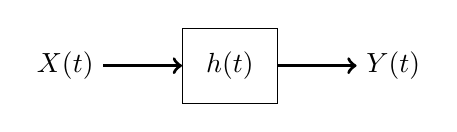
\begin{tikzpicture}[scale=1.0,transform shape]
        \tikzstyle{rectblock}=[rectangle, draw, inner sep=3mm]
        \node (X) {$X(t)$};
        \node[rectblock, right = 1cm of X] (h) {$h(t)$};
        \node[right = 1cm of h] (Y) {$Y(t)$};
        \draw [->,very thick] (X) -- (h);
        \draw [->,very thick] (h) -- (Y);
      \end{tikzpicture}
      \end{figure}
  \end{itemize}
  \normalsize
\end{frame}

%% Frame %%
\begin{frame}{White Gaussian Noise}
  \footnotesize
  \pause
  \begin{definition}[]
    A zero mean WSS Gaussian random process with power spectral density
    \begin{equation*}
      S_n(f) = \frac{N_0}{2}.
    \end{equation*}
    \pause $\frac{N_0}{2}$ is termed the two-sided PSD and has units Watts per Hertz.
  \end{definition}
  \pause
  \begin{block}{Remarks}
    \begin{itemize}
      \item Autocorrelation function $R_n(\tau) = \pause \frac{N_0}{2}\delta(\tau)$
      \item \pause \alert{Infinite Power!}\pause \ \  Ideal model of Gaussian noise occupying more bandwidth than the signals of interest.
    \end{itemize}
  \end{block}
  \normalsize
\end{frame}

%% Frame %%
\begin{frame}{White Gaussian Noise through Correlators}
  \footnotesize
  \begin{itemize}
    \pause
    \item Consider the output of a correlator with WGN input
      \begin{equation*}
        Z = \int_{-\infty}^{\infty} n(t) u(t) \ dt = \langle n, u\rangle
      \end{equation*}
      where $u(t)$ is a deterministic finite-energy signal
    \pause
    \item $Z$ is a Gaussian random variable
    \pause
    \item The mean of $Z$ is
      \pause
      \begin{equation*}
        E[Z] = \pause \int_{-\infty}^{\infty} E\left[n(t)\right] u(t) \ dt = \pause 0
      \end{equation*}
    \pause
    \item The variance of $Z$ is \pause
      \begin{eqnarray*}
        \text{var}(Z) & = & \pause E\left[ \left(\langle n, u \rangle \right)^2 \right]  = \pause E \left[ \int n(t) u(t) \ dt \int n(s) u(s) \ ds \right] \\
        & = & \pause \int \int u(t) u(s) E\left[ n(t) n(s) \right] \ dt \ ds \\
        & = & \pause \int \int u(t) u(s) \frac{N_0}{2} \delta(t-s) \ dt \ ds \\
        & = & \pause \frac{N_0}{2} \int u^2(t) \ dt = \pause \frac{N_0}{2} \lVert u \rVert^2
      \end{eqnarray*}
  \end{itemize}
  \normalsize
\end{frame}

%% Frame %%
\begin{frame}{White Gaussian Noise through Correlators}
  \footnotesize
  \begin{block}{Proposition}
  Let $u_1(t)$ and $u_2(t)$ be linearly independent finite-energy signals and let $n(t)$ be WGN with PSD $S_n(f) = \frac{N_0}{2}$. \pause Then $\langle n, u_1 \rangle$ and $\langle n, u_2 \rangle$ are jointly Gaussian with covariance \pause
      \begin{equation*}
        \text{cov}\left( \langle n, u_1 \rangle, \langle n, u_2 \rangle \right) = \frac{N_0}{2} \langle u_1, u_2 \rangle.
      \end{equation*}
  \end{block}
  \pause
  \begin{block}{Proof}
     To prove that $\langle n, u_1 \rangle$ and $\langle n, u_2 \rangle$ are jointly Gaussian, consider a non-trivial linear combination $a\langle n, u_1 \rangle + b\langle n, u_2 \rangle$ 
      \begin{equation*}
        a\langle n, u_1 \rangle +b \langle n, u_2 \rangle  = \pause \int n(t) \left[au_1(t) + bu_2(t)\right] \ dt.
      \end{equation*}
    \pause This is the result of passing $n(t)$ through a correlator. So it is a Gaussian random variable.
  \end{block}
  \normalsize
\end{frame}

%% Frame %%
\begin{frame}{White Gaussian Noise through Correlators}
  \footnotesize
  \begin{block}{Proof (continued)}
      \begin{eqnarray*}
        \text{cov}\left( \langle n, u_1 \rangle, \langle n, u_2 \rangle \right) & = & \pause E\left[ \langle n, u_1 \rangle \langle n, u_2 \rangle \right] \\
        & = & \pause E \left[ \int n(t) u_1(t) \ dt \int n(s) u_2(s) \ ds \right] \\
        & = & \pause \int \int u_1(t) u_2(s) E\left[ n(t) n(s) \right] \ dt \ ds \\
        & = & \pause \int \int u_1(t) u_2(s) \frac{N_0}{2} \delta(t-s) \ dt \ ds \\
        & = & \pause \frac{N_0}{2} \int u_1(t) u_2(t) \ dt \\
        & = & \pause \frac{N_0}{2} \langle u_1, u_2 \rangle
      \end{eqnarray*}
  \end{block}
  If $u_1(t)$ and $u_2(t)$ are orthogonal, \pause $\langle n, u_1 \rangle$ and $\langle n, u_2 \rangle$ are independent.
  \normalsize
\end{frame}


\begin{frame}{}
\vfill
\begin{center}
Thanks for your attention
\end{center}
\vfill
\end{frame}
\end{document}
